%-------------------------------------------------------------------------------
\subsubsection{Dynamique de population à trois classes : mâles, femelles et couples}
%-------------------------------------------------------------------------------

On considère une population sexuée panmictique, au sein de laquelle on désigne
respectivement par $x(t)$, $y(t)$ et $z(t)$ les densités au temps $t$ de femelles flottantes, de mâles flottants, et de couples. On suppose que la dynamique de la population respecte le système dynamique suivant
\begin{equation} \label{eq:Dyn3Pop}
  \left\{\begin{array}{rcl}
          \dot x(t) & = & - \alpha x y + r z, \\
          \dot y(t) & = & - \alpha x y + r z, \\
          \dot z(t) & = & + \alpha x y - c z^2,
          \end{array} \right.
\end{equation}
où les coefficients $\alpha$, $r$ et $c$ sont strictement positifs.
\begin{enumerate}
  \item Interpréter ces équations et la signification de chacun des coefficients $\alpha$, $r$ et $c$.
  \solution{Les mâles et femelles flottant(e)s s'apparient pour former des couples : 
  \begin{itemize}
    \item $\alpha$ est le taux de formation des couples, 
    \item $r$ est le taux de natalités de mâles et des femelles (supposés égaux),
    \item $c$ est le taux de mortalité des couples.
  \end{itemize}
  }
  \item En notant $S = x(0) - y(0)$, montrer que $x(t) - y(t) = S$ pour tout temps $t$. En
  déduire les fonctions $y$ et $z$ satisfont le système 
  \begin{equation} \label{eq:Dyn3Pop2}
    \left\{\begin{array}{rcl}
            \dot y(t) & = & - \alpha (y^2 + Sy) + r z, \\
            \dot z(t) & = & + \alpha (y^2 + Sy) - c z^2.
            \end{array} \right.
  \end{equation}
  Dans la suite on supposera que $S > 0$.
  \solution{On remarque que
  $$
  \dot x(t) - \dot y(t) = 0,
  $$
  ce qui implique que la différence $x(t) - y(t)$ reste constante au cours du temps et égale à $x(0) - y(0) = S$. \\
  On peut donc remplacer $x(t) = y(t) + S$ dans le système \eqref{eq:Dyn3Pop} pour obtenir le système \eqref{eq:Dyn3Pop2}.}
  \item Déterminer les points d'équilibre du système \eqref{eq:Dyn3Pop2}.
  \solution{
  \begin{itemize}
    \item $(y^* = 0, z^* = 0)$ est un équilibre (trivial).
    \item $(y = -S, z^* = 0)$ n'est pas un équilibre intéressant du point de vue du modèle car on s'intéresse aux effectifs positifs ou nuls. 
    \item Si on suppose $({y^*}^2 + Sy^*) \neq 0$, il vient
    $$
    \alpha({y^*}^2 + Sy^*) = rz^* = c{z^*}^2 
    \qquad \Rightarrow \qquad 
    z^* = r / c
    $$
    et $y^*$ doit vérifier
    $$
    {y^*}^2 + Sy^* - \frac{r^2}{\alpha c} = 0,
    $$
    dont le discriminant est 
    $$
    \Delta =  S^2 + \frac{4 r^2}{\alpha c} > S^2,
    $$
    et dont la seule solution positive est
    $$
    y^* = \frac{\sqrt{\Delta} - S}2.
    $$
    On a donc 4 points d'équilibres : 
    $$
    (0, 0), \qquad
    (-S, 0), \qquad 
    \left(\frac{\sqrt{\Delta} - S}2, \frac{r}c\right), \qquad
    \left(\frac{-\sqrt{\Delta} - S}2, \frac{r}c\right)
    $$
    dont les seuls pertinent pour le modèle sont ceux qui se situent dans le cadrant positif, c'est-à-dire
    $$
    (y=0, z=0), \qquad
    \left(y=\frac{\sqrt{\Delta} - S}2, z=\frac{r}c\right).
    $$
  \end{itemize}
  }
  \item \'Ecrire la matrice jacobienne du système \eqref{eq:Dyn3Pop2} et étudier la nature du ou des équilibres non triviaux.
  \solution{La jacobienne vaut
  $$
  J F = \left[\begin{array}{rr}
              -2 \alpha y - \alpha S & r \\ 2 \alpha y + \alpha S & -2 c z
            \end{array}\right]
  $$
  \begin{description}
    \item[En $(0, 0)$ :] on a 
    $$
    J_{(0, 0)} F = \left[\begin{array}{rr}
                - \alpha S & r \\ \alpha S & 0
              \end{array}\right]
    \qquad \Rightarrow \qquad
    P(\lambda) = \lambda^2 + \alpha S \lambda - r \alpha S
    $$
    où
    $$
    \Delta_0 = \alpha^2 S^2 (1 + 4 r / (\alpha S)) > \alpha^2 S^2.
    $$
    Les deux valeurs propres
    \begin{align*}
    \lambda_1 
    & = \frac{-\alpha S + \sqrt{\Delta_0}}{2}
    = \alpha S \left(-1 + \sqrt{1 + \delta}\right), 
    \\
    \lambda_2 
    & = \frac{-\alpha S - \sqrt{\Delta_0}}{2}
    = \alpha S \left(-1 - \sqrt{1 + \delta}\right), 
    \end{align*}
    (où $\delta = 4r/\alpha S$) sont donc de signe opposé : $(0, 0)$ est stable dans une direction et instable dans une autre. \\
    Il est alors intéressant de savoir quelle direction propre concerne le cadrant positif. On cherche pour cela les vecteurs propres en écrivant que $(u, v)$ est un vecteur propre de $J_{(0, 0)} F$ associé à $ \lambda$ ssi
    \begin{align*}
      J_{(0, 0)} F \cdot [u \; v]^\top = \lambda [u \; v]^\top
      \qquad \Leftrightarrow \qquad
      \left\{\begin{array}{rcl}
              - \alpha S u + r v & = & \lambda u \\
              \alpha S u & = & \lambda v
             \end{array}\right. .
    \end{align*}
    La second équation impose donc
    $$
    \alpha S u = \alpha S \left(-1 \pm \sqrt{1 + \delta}\right) v.
    $$
    $u$ et $v$ sont donc de même signe pour $\lambda_1 > 0$ (direction instable) et de signe opposé pour $\lambda_2 < 0$ (direction stable). $(0, 0)$ n'est donc pas un point attracteur dans le cadrant positif.
    \item[En $(y^* = \sqrt{\Delta} - S)/2, z^* = r/c)$ :] on a 
    $$
    J_{(y^*, z^*)} F = \left[\begin{array}{rr}
                - \alpha \delta & r \\ \alpha \delta & -2 r
              \end{array}\right]
    \qquad \Rightarrow \qquad
    P(\lambda) = \lambda^2 + (\alpha \delta + 2r) \lambda - r \alpha \delta,
    $$
    en notant $\delta = 2(\sqrt{\Delta} - S) + S = 2\sqrt{\Delta} - S > 0$. On a cette fois
    $$
    \Delta^* 
    = \frac12 \left((\alpha \delta + 2r)^2 - 4 r \alpha \delta\right)
    = \frac12 (\alpha \delta - 2r)^2 \geq 0,
    $$
    soit
    $$
    \lambda = \frac12 \left(-(\alpha \delta + 2r) \pm \sqrt{\Delta^* }\right) \leq 0
    $$
    car, les coefficients $\alpha$, $r$ et $c$ étant tous positifs,
    $$
    \frac12 (\alpha \delta - 2r)^2 < (\alpha \delta + 2r)^2.
    $$
    $(y^* = \sqrt{\Delta} - S)/2, z^* = r/c)$ est donc un équilibre stable.
    
  \end{description}
  $$
  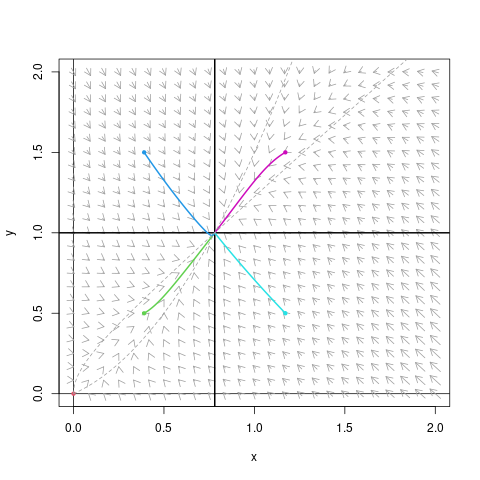
\includegraphics[width=.5\textwidth]{DynPopMaleFemelleCouple.png}
  $$
  }
\end{enumerate}

